\documentclass[11pt]{article}
\usepackage{graphicx}
\graphicspath{{./Images/}}
\usepackage{setspace}
\usepackage{subcaption}
\usepackage{multirow}
\usepackage{diagbox}
\usepackage{color, colortbl}
\definecolor{yellow}{rgb}{1,1,0.25}
\usepackage[left=3.2cm, right=3.2cm, top=3cm]
{geometry}
\setstretch{1.5}
\usepackage[bottom]{footmisc}
\begin{document}
\title{Predicting Movie Review Sentiment \\
Based On Classifier And Ridge Regression}
\author{Qiao Qiao\\qqiao1@hawk.iit.edu\\Math569}
\maketitle
\newpage

\section*{1.Problem Description}
\subsection*{1.1 Background}
\hspace{1.5em}The goal of my project is to build a text classifier to determine whether a movie review is expressing positive or negative sentiment.

I'll write code to preprocess the data in different ways (creating different features), then compare the cross-validation accuracy of each approach. Meanwhile,I'll compute accuracy on a test set and do some analysis of the errors.

The project is coded in Python and use statistical learning techniques to provide a prediction. 
$\mathbf{P}(\omega)=\mathbf{P}\left(\omega_{1} \cup \omega_{2} \cup \cdots \cup \omega_{k}\right)=\prod_{i=1}^{k} \mathbf{P}_{\mathbf{T}_{i}}\left(\omega_{i}\right)$

\section*{2.Data Source}
\subsection*{2.1 Getting the Dataset}
\hspace{1.5em}The data come from the website IMDB.com.

The "Large Movie Review Dataset" shall be used for this project. The dataset is compiled from a collection of 50,000 reviews from IMDB on the condition there are no more than 30 reviews per movie. The numbers of positive and negative reviews are equal. Negative reviews have scores less or equal than 4 out of 10 while a positive review have score greater or equal than 7 out of 10. Neutral reviews are not included. The 50,000 reviews are divided evenly into the training and test set.

After I collected data, I walked all subdirectories and read all the text files and labels. Then I defined a function called "tokenize", in this function, I tokenize all text to strings, and let the string be converted to lowercase.

\subsection*{2.2 Data Processing}
\hspace{1.5em}The training dataset has two sub-directories pos/ for positive texts and neg/ for negative ones. Use only these two directories. The first task is to combine both of them to a single csv file, the csv file has three columns, ``row number",``text" and ``polarity". The column ``text" contains review texts and the column ``polarity" consists of sentiment labels, 1 for positive and 0 for negative. The file imdbtr.csv is an output of this preprocessing. In addition, common English stopwords should be removed. An English stopwords reference (`stopwords.en') is given in the code for reference.

Initially the dataset was divided into two subsets containing 25,000 examples each for training and testing. I found this division to be sub-optimalas the number of training examples was very small and leading to under-fitting. Then I tried to redistribute the examples as 40,000 for training and 10,000 for testing. While this produced better models, it also led to over-fitting on training examples and worse performance on the test set. Finally, I decided to use Cross-Validation in which the complete dataset is divided into multiple folds with different samples for training and validation each time and the final performance statistic of the classifieris averaged over all results. This improved the accuracy of my models across the boards.
\section*{3.Predictive Analysis}
\subsection*{3.1 Exploratory Analysis}
\hspace{1.5em}One of the starting points while working with review text is to calculate the average size of reviews to get some insight on quality of reviews.  The average number of words per review is around 120. The Figure 1 clearly indicate the variation of the word count for each review. From this information I deduced that in general people tend to write pretty descriptive reviews for movies and as such this is  good topic for sentiment analysis. Also, people generally write reviews when they have strong opinions about a movie; they either loved it or hated it.
\begin{figure}[h!]
  \centering
    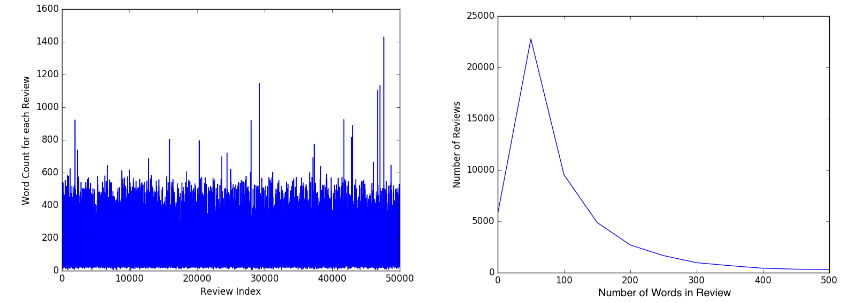
\includegraphics[width=1.2\linewidth]{1.png}
    \caption{}
\end{figure}

Apart from the word count per review another interesting metric was occurrence count of words across reviews. Some words have higher occurrence counts as compared to others depending on their relative importance. Table 1 is the list of 20 most occurring words in negative and positive reviews along with a graph showing variability of word occurrences across all reviews. Also, the average word occurrence count was around 33 over all 50000 reviews.From all this information and the below graphs, it is clear that “Bag of Words” is not a very good model for doing sentiment analysis of reviews because similar words have high counts in both positive and negative reviews. Also, overall number of unique words is huge(1,63,353) across all the reviews and hence I use only top 50,000 and 1,00,000 of these during training. Also, this realization prompted me to move to other methods of feature extraction like cross validation and logistic regression.
\begin{center}
\begin{tabular}{|c|c|c|c|}
\hline
 \multicolumn{2}{|c|}{Negative Reviews} 
 &\multicolumn{2}{|c|}{Positive Reviews} \\
 \hline
Movie &  Film & Film & Movie \\
\hline
Like&Even&Film&Movie\\
\hline
Good&Bad&Great&Story\\
\hline
Would&Really&See&Time\\
\hline
Time&See&Well&Also\\
\hline
Don't&Get&Really&Would\\
\hline
Much&Story&Even&Much\\
\hline
People&Could&First&Films\\
\hline
Make&Made&Love&People\\
\hline
Movies&First&Best&Get\\
\hline
\end{tabular}
\\
\bigskip
Table 1
\end{center}
\begin{figure}[h!]
  \centering
    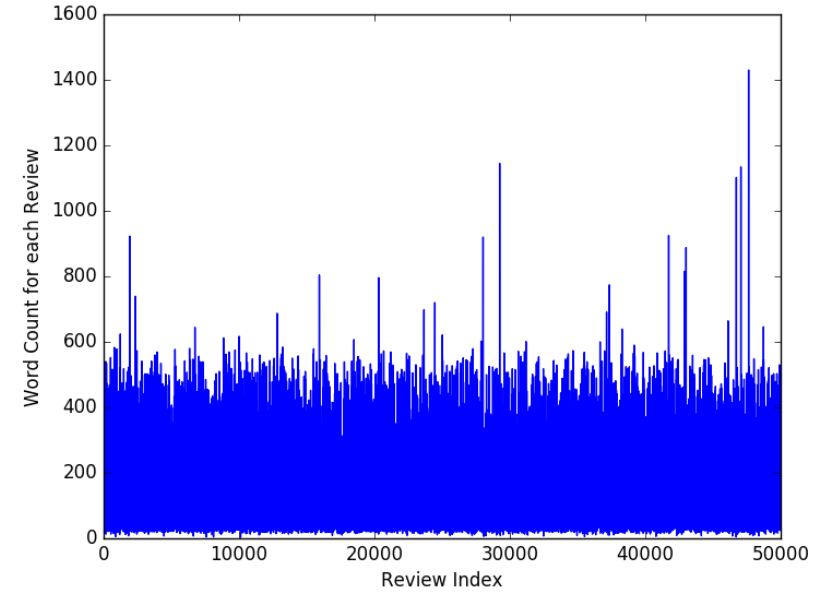
\includegraphics[width=\linewidth]{2.png}
    \caption{}
\end{figure}

\subsection*{3.2 Feature Extraction}
\subsubsection*{3.2.1 Bag of Words}
\hspace{1.5em}This is a typical way for word representation in any text mining process. I first calculated the total word counts for each word across all the reviews and then used this data to create different feature representations. As the total number of words in the dictionary was huge (more than1,60,000) the first feature set was created using only the 50,000 most frequent words according to their occurrence. Another feature set was created in a similar fashion but using top 1,00,000 words. In addition to this,I created another bag of words representation using all words that occurred at least twice across the whole dataset. This ensured that I remove most of the misspelled words. Also,words which occurred only once in the dataset would contribute nothing to the classifier. Another feature representation was created along the same lines but with words occurring at least 5 times. The size of these 2 features representations was roughly 34,000 and 76,000 respectively. 
\subsubsection*{3.2.2 Token pair features}
\hspace{1.5em}Compute features indicating that two words occur near each other within a window of size k. 

For example [a, b, c, d] with k=3 will consider the windows: [a,b,c], [b,c,d]. In the first window,a\_b, a\_c, and b\_c appear; in the second window,b\_c, c\_d, and b\_d appear. 
\subsubsection*{3.2.3 Lexicon Features}
\hspace{1.5em}Lexicon features indicates how many time a token appears that matches either the neg\_words or pos\_words. The matching should ignore case.

I defined neg\_words and pos\_words.

neg\_words = set(['bad', 'hate', 'horrible', 'worst', 'boring'])

pos\_words = set(['awesome', 'amazing', 'best', 'good', 'great', 'love', 'wonderful'])

\subsection*{3.3 Cross Validation Accuracy}
\hspace{1.5em}Compute the average testing accuracy over k folds of cross-validation. I use sklearn's KFold class, LogisticRegression classifier and a csr\_matrix of features here.

Then I enumerate all possible classifier settings and compute the cross validation accuracy for each setting. I use this to determine which setting has the best accuracy.

For each setting, construct a LogisticRegression classifier and compute its cross-validation accuracy for that setting.

Here are my result:

\textbf{best cross-validation result:}

$\{'punct': True, 'features': [<function token\_pair\_features \; at \; 0x7f618f4d31e0>, <function lexicon\_features \;at\; 0x7f618f4d3268>], 'min\_freq': 2, 'accuracy': 0.7700000000000001\}$

\textbf{worst cross-validation result:}

$\{'punct': True, 'features': [<function lexicon\_features \;at\; 0x7f618f4d3268>], 'min\_freq': 2, 'accuracy': 0.6475\}$

To determine how important each model setting is to overall accuracy,I compute the mean accuracy of all combinations with a particular setting. Here is the result.

$\textbf{Mean Accuracies per Setting:}\\
features=token\_pair\_features \;lexicon\_features: 0.75167\\
features=token\_features\; token\_pair\_features\; lexicon\_features: 0.74583\\
features=token\_features \;token\_pair\_features: 0.73542\\
features=token\_pair\_features: 0.72875\\
min\_freq=2: 0.72268\\
punct=False: 0.72024\\
min\_freq=5: 0.71857\\
punct=True: 0.70833\\
min\_freq=10: 0.70161\\
features=token\_features\; lexicon\_features: 0.69708\\
features=token\_features: 0.69000\\
features=lexicon\_features: 0.65125$

Figure 3 shows all accuracies in ascending order of accuracy.
\begin{figure}[h!]
  \centering
    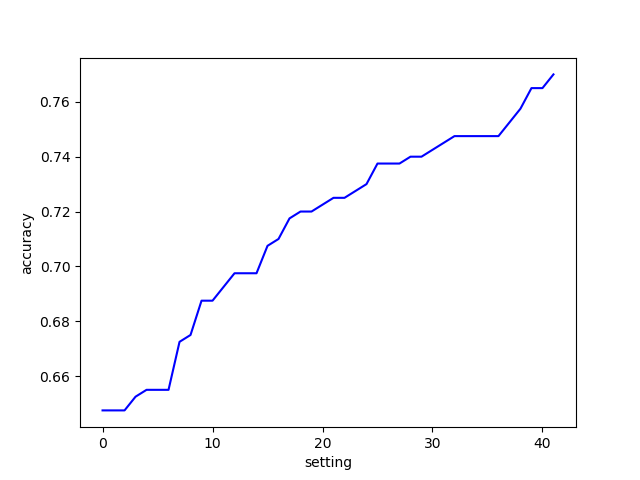
\includegraphics[width=\linewidth]{3.png}
    \caption{}
\end{figure}

\subsection*{3.4 TOP MISCLASSIFIED TEST DOCUMENTS}
\hspace{1.5em}There exists some testing documents that are misclassified by the
largest margin. By using the .predict\_proba function of LogisticRegression, I get the predicted probabilities of each class for each instance. I first identify all incorrectly classified documents, then sort them in descending order of the predicted probability for the incorrect class.

\textbf{Figure 4 is part of my result:}
\begin{figure}[h!]
  \centering
    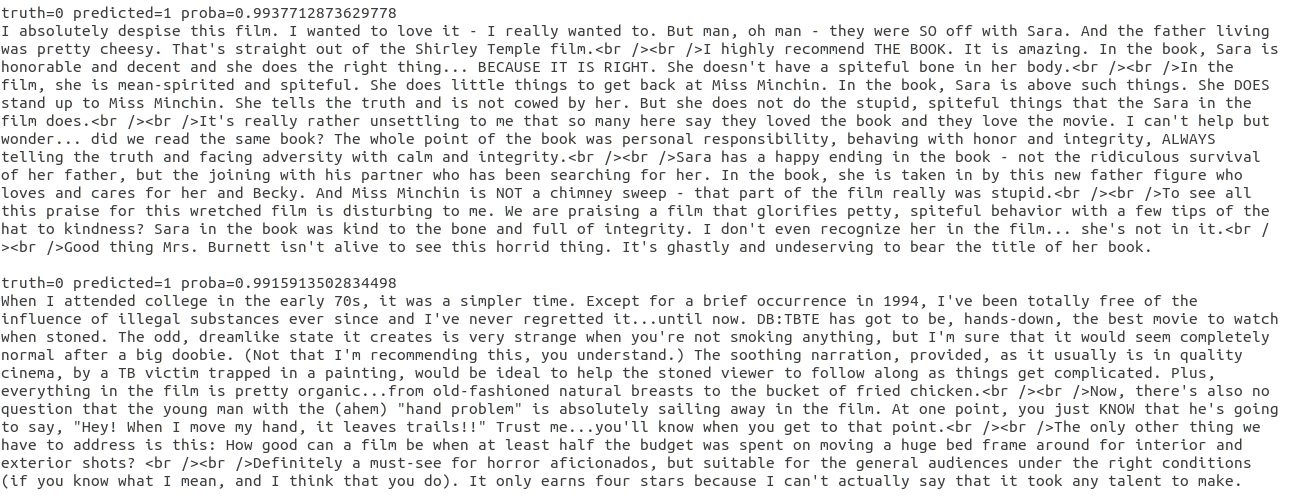
\includegraphics[width=\linewidth]{4.png}
    \caption{}
\end{figure}

\subsection*{3.5 Model Improvements}
\hspace{1.5em}Looking at the top errors, I think I can modify my classifier to improve accuracy ,it could be features, tokenization, or something else.

(1) Tokenization:

After I looked at these misclassified documents,I relized a common problem in sentiment analysis is negation. E.g., ``This movie is not good" ,``This movie is good, but..." and ``This movie is good" will have very similar feature vectors. However, the term good in the first two sentence is clearly being used differently than in the last sentence. 

I can change my tokenize function:

For example,whenever the term `not' or `but' appears, change the two subsequent tokens to have the prefix `not\_' or `but\_' prior to the token.

(2) Increase the number of folds:

When number of folds increases for a fixed amount of data, number of data within each fold decreases. Hence, less data is available for testing, and more data is available for training. 

It trains the model more and tests the model with less data per fold. Hence, accuracy increases.

I tried to increase the number of folds from 5 to 10, then my testing accuracy change from 0.727500 to 0.780000, all ``Mean Accuracies per Setting" increase,
``worst cross-validation result" is the same with original, but it's accuracy increases from 0.6475 to 0.6525.


\section*{4.Conclusion}
\hspace{1.5em}From the results above, I infer that for my problem statement, Logistic Regression Model with feature set using mixture of unigrams is best.

One of the major improvements that can be incorporated as I move ahead in this project is to merge  words  with  similar  meanings  before  training  the  classifiers.Another  point  of improvement can be to model this problem as a multi-class classification problem where I classify the sentiments of reviewer in more than binary fashion like “Happy”, “Bored”, “Afraid”, etc.This problem can be further remodeled as aregression problem where I can predict the degree of affinity for the movie instead of complete like/dislike. 
\newpage
\section*{Reference}
1. Andrew L. Maas, Raymond E. Daly. Learning Word Vectors for Sentiment Analysis\\
2. R. Collobert and J. Weston.  A unified architecture for natu-ral language processing: Deep neural networks with multitasklearning.  In Proceedings of the 25th international conference on Machine learning, pages 160–167. ACM, 2008. \\
3. Logistic regression: the .predict\_proba function of LogisticRegression \textit{https://goo.gl/4WXbYA/}\\
4. Alejandro Pelaez, Talal Ahmed, Mohsen Ghassem (2015). Sentiment analysis of IMDb movie reviews

\end{document}